% Source for images/chapter_menu.png, the two chapter menus in Chapter 4.
% The entries are what ebook-convert makes for this book with each setting.
% To remake the PNG:
%   cd images && pdflatex chapter_menu.tex && pdftoppm -png -r 300 -gray -singlefile chapter_menu.pdf chapter_menu && magick chapter_menu.png -colorspace Gray chapter_menu.png
\documentclass[border=8pt]{standalone}
\usepackage[T1]{fontenc}
\usepackage[scaled]{helvet}
\renewcommand{\familydefault}{\sfdefault}
\usepackage{tikz}

\newcommand{\ch}[1]{\textbf{#1}\\}
\newcommand{\se}[1]{\hspace*{1.2em}#1\\}
\newcommand{\fl}[1]{#1\\}
\newcommand{\gap}{\hspace*{1.2em}\ldots\\}

\begin{document}
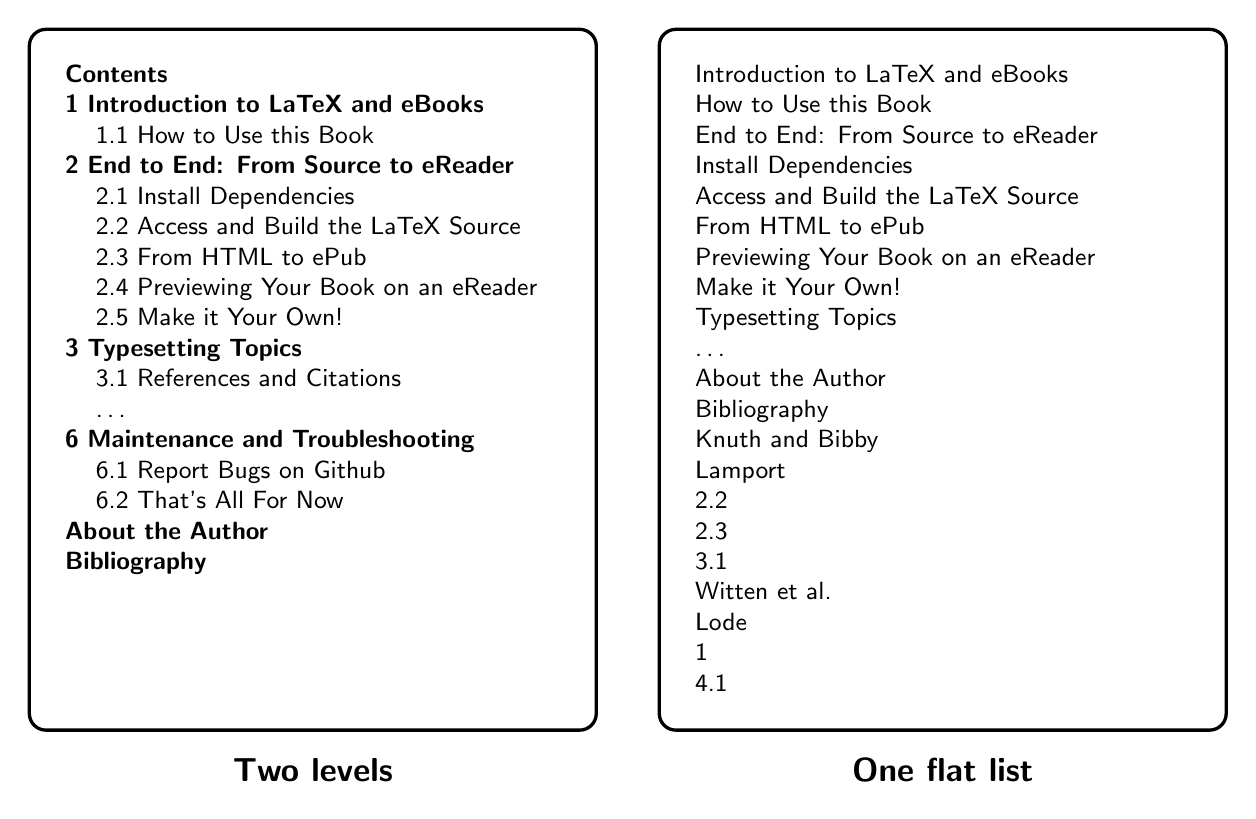
\begin{tikzpicture}[
    screen/.style={draw, line width=1.2pt, rounded corners=6pt, minimum width=7.2cm,
      minimum height=8.9cm, anchor=north, inner sep=10pt},
    menu/.style={anchor=north west, align=left, font=\small, text width=6.4cm},
  ]
  \node[screen] (left) at (0, 0) {};
  \node[screen] (right) at (8, 0) {};
  \node[menu] at ([xshift=10pt, yshift=-10pt]left.north west) {
    \ch{Contents}
    \ch{1 Introduction to LaTeX and eBooks}
    \se{1.1 How to Use this Book}
    \ch{2 End to End: From Source to eReader}
    \se{2.1 Install Dependencies}
    \se{2.2 Access and Build the LaTeX Source}
    \se{2.3 From HTML to ePub}
    \se{2.4 Previewing Your Book on an eReader}
    \se{2.5 Make it Your Own!}
    \ch{3 Typesetting Topics}
    \se{3.1 References and Citations}
    \gap
    \ch{6 Maintenance and Troubleshooting}
    \se{6.1 Report Bugs on Github}
    \se{6.2 That's All For Now}
    \ch{About the Author}
    \ch{Bibliography}
  };
  \node[menu] at ([xshift=10pt, yshift=-10pt]right.north west) {
    \fl{Introduction to LaTeX and eBooks}
    \fl{How to Use this Book}
    \fl{End to End: From Source to eReader}
    \fl{Install Dependencies}
    \fl{Access and Build the LaTeX Source}
    \fl{From HTML to ePub}
    \fl{Previewing Your Book on an eReader}
    \fl{Make it Your Own!}
    \fl{Typesetting Topics}
    \fl{\ldots}
    \fl{About the Author}
    \fl{Bibliography}
    \fl{Knuth and Bibby}
    \fl{Lamport}
    \fl{2.2}
    \fl{2.3}
    \fl{3.1}
    \fl{Witten et al.}
    \fl{Lode}
    \fl{1}
    \fl{4.1}
  };
  \node[below=6pt, font=\large\bfseries] at (left.south) {Two levels};
  \node[below=6pt, font=\large\bfseries] at (right.south) {One flat list};
\end{tikzpicture}
\end{document}
